\documentclass[tikz,border=7pt]{standalone}
\usepackage[e]{esvect}
\usetikzlibrary{calc}
\tikzset{
  line/.style = {
    shorten <=-3mm, shorten >=-3mm
  },
  vector/.style = {
    thick,-latex
  },
  dot/.style = {
    insert path={
      node[scale=2]{.}
    }
  },
}
\begin{document}
  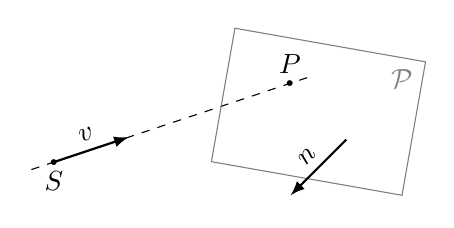
\begin{tikzpicture}
    \path
      (0,0) coordinate (S)
      (3,1) coordinate (P)
      ($(S)!1cm!(P)$) coordinate (v)
      (2.3,1.7) coordinate (B)
      ($(B)!3cm!(P)$) coordinate (A)
      ($(B)!2cm!(P)$) coordinate (N)
      ($(N)!1cm!90:(B)$) coordinate (n)
    ;
    \draw
      (S) edge[line, dashed] (P)
    ;
    \draw[gray]
      {[rotate=-10](A) rectangle (B)}
    ;
    \draw
      (S) edge[vector] node[above, sloped]{$\vv{v}$} (v)
      (N) edge[vector] node[above, sloped]{$\vv{n}$} (n)
    ;
    \path
      (S) [dot] node[below]{$S$}
      (P) [dot] node[above]{$P$}
      (A|-B) node[gray, below=4mm]{$\mathcal{P}$}
    ;

  \end{tikzpicture}
\end{document}
